\documentclass[12pt, letterpaper]{article}
\usepackage{amsmath}
\usepackage{tikz}
\usepackage{pgfplots}
\usetikzlibrary{patterns}
\pgfplotsset{compat=1.18}
\title{Applied 354 Lecture Notes}
\author{Anthony Durrer}
\newcommand{\un}[1]{\underline{#1}}
\newcommand{\partFrac}[2]{\frac{\partial #1}{\partial #2}}
\begin{document}
	\maketitle

	\section{Notes: 02 Aug}
	\paragraph{Calculate Divergance Theorem}
		Given the vector field, where $z=0$:
		\footnote{hello my name is periwinkle and im so cute and hungry}
		\begin{equation}
			\underline{v}=3y^{2}z\underline{i} + 2y^{2}\underline{j} + yz^{2}\underline{k}
		\end{equation}
		\begin{equation}
			\underline{v} = 2y^{2}\underline{j}
		\end{equation}
		The divergance theorem is given by:
		\begin{equation}
			\iint_A \nabla \cdot \underline{v} dA  = \oint \underline{n} \cdot \underline{v} dr
		\end{equation}
		Calculating the inside of the LHS:
		\begin{equation}
			\nabla \cdot \un{v} = \un{j} \partFrac{}{y} \cdot 2y^{2} \un{j} = 4y
		\end{equation}
		Therefor calculating LHS:
		\begin{equation}
			\iint_A \nabla \cdot \underline{v} \; dA  = \int_{2}^{3} \int_2^4 4y \;dxdy
		\end{equation}
		\begin{equation}
			\iint_A \nabla \cdot \underline{v} \; dA  = \Big| 8 \frac{y^2}{2} \Big|_2^3 = 20
		\end{equation}

		Calculating the RHS, using the graphic finding the normal vectors to each side. Only two terms
		are present as i dot j will be zero, so the verticals are zero.

		\begin{equation}
			\oint \underline{n} \cdot \underline{v} dr = \int_2^4 -\un{j} \cdot 2y^2\un{j} dx + \int_2^4 \un{j} \cdot 2y^2\un{j} dx 
		\end{equation}
		Using Figure:\ref{fg:1} replacing the y values from the graphic, 2 and 3 respectivly
		\begin{equation}
			= \int_2^4 -8 dx + \int_2^4 18 dx = 20
		\end{equation}
		Therefor RHS = LHS
		\begin{figure}[h]
			\centering
			\caption{Vector Field Figure}
			\label{fg:1}
			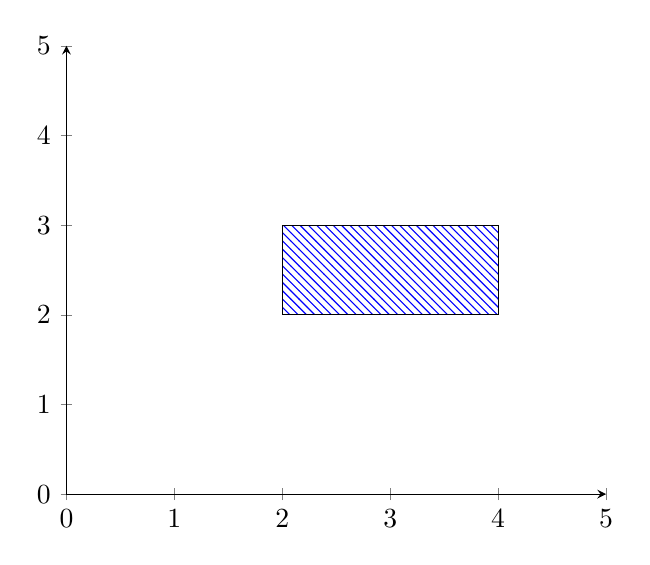
\begin{tikzpicture}
			\begin{axis}[xmin=0, xmax=5, ymin=0, ymax=5, axis x line=bottom, axis y line=left]
				\draw[pattern=north west lines, pattern color=blue] (2,2) rectangle (4,3);
			\end{axis}
			\end{tikzpicture}
		\end{figure}


	\paragraph{Calculate Stokes Integral Theorem} for the velocity field $v=x \un{j}$
\end{document}
